\documentclass[11pt]{article}
\usepackage[margin=1in]{geometry}
\usepackage{amsmath,amssymb,amsthm}
\usepackage{booktabs,array,longtable,tabularx}
\usepackage{graphicx}
\usepackage{microtype}
\usepackage{xcolor}
\usepackage[font=small,labelfont=bf]{caption}
\usepackage{enumitem}
\usepackage{url}
\usepackage[hidelinks]{hyperref}
\usepackage{natbib}
\usepackage{amsfonts}
\usepackage{pifont}
\renewcommand{\checkmark}{\ding{51}}
\newcommand{\auxTwelveD}{16}
\newcommand{\auxTwelveC}{1}
\newcommand{\auxTwelveH}{3}
\newcommand{\auxTwelveFixed}{15}
\newcommand{\auxTwelveLabels}{16}
\newcommand{\auxTwelveExampleForm}{-\tfrac{1}{2}T\,x_{3} - T\,x_{4} + x_{10}}
\newcommand{\auxTwelveExampleClause}{2}
\newcommand{\auxTwelveExampleVar}{10}
\newcommand{\auxTwelveHone}{-12561/32}
\newcommand{\auxTwelveHtwo}{-9664}
\newcommand{\auxTwelveCount}{736}
\newcommand{\directFourteenSums}{580}
\newcommand{\directFourteenClauseEvals}{18,104,320}
\newcommand{\directFourteenMinutes}{9.2}
\newcommand{\directFourteenCount}{3108}
\newcommand{\toyRunsCount}{12}
\newcommand{\auxSixQ}{7}
\newcommand{\auxSixM}{15}
\newcommand{\auxSixSums}{1,458}
\newcommand{\toyPointsCertified}{116}
\newcommand{\compTwoThirds}{$n = 1,000$: largest 83--109, $n^{2/3} = 100$; $n = 4,000$: largest 196--229, $n^{2/3} = 252$; $n = 16,000$: largest 685--1656, $n^{2/3} = 635$}
\newcommand{\fibreInstances}{19}
\newcommand{\fibreDictRatioMin}{0.02}
\newcommand{\fibreDictRatioMax}{1.23}
\newcommand{\fibreBucketRatioMin}{0.38}
\newcommand{\fibreBucketRatioMax}{103.6}
\newcommand{\fibreDensityMin}{4}
\newcommand{\fibreDensityMax}{24}
\newcommand{\fibreSubcritMin}{0.4}
\newcommand{\fibreSubcritMax}{103.6}
\newcommand{\fibrePackedOverDictMax}{57}
\newcommand{\fibreBestSubcritMin}{14.6}
\newcommand{\fibreBestSubcritMax}{299.9}
\newcommand{\fibreBestRtwoMax}{7.7}
\newcommand{\fibrePackedFasterCount}{5}
\newcommand{\fibreExactChecks}{3}
\newcommand{\multirowPB}{43.0}
\newcommand{\multirowTwo}{50.8}
\newcommand{\multirowPBentries}{37}
\newcommand{\multirowTwoEntries}{100}
\newcommand{\gridSixSixMs}{37.9}
\newcommand{\encRatioMin}{0.6}
\newcommand{\encRatioMax}{1,083}
\newcommand{\encRatioGridMax}{134}
\newcommand{\encRatioRandomMax}{1,083}
\newcommand{\histOverPlainMin}{1.2}
\newcommand{\histOverPlainMax}{1.3}
\newcommand{\encFortyTwentySeconds}{356}
\newcommand{\encFortyTwentyNodes}{97,698}
\newcommand{\encFortyTwentyComp}{649}
\newcommand{\encFortyTwentyRatio}{1,083}
\newcommand{\histFortyMs}{329}
\newcommand{\histFortyEntries}{26}
\newcommand{\gridEightTotal}{660,647,962,955}
\newcommand{\gridEightMs}{608}
\newcommand{\gridEightSizes}{33}
\newcommand{\gridSixEncComp}{323}
\newcommand{\gridSixEncRatio}{134}
\newcommand{\expFirstPositive}{26}
\newcommand{\expThresholdLambda}{44{,}318{,}976}
\newcommand{\expThresholdLog}{25.4}
\newcommand{\expShareA}{14.6}
\newcommand{\expRatioA}{6}
\newcommand{\expShareB}{2.0}
\newcommand{\expRatioB}{48}
\newcommand{\expShareC}{0.69}
\newcommand{\expRatioC}{144}
\newcommand{\expShareD}{0.51}
\newcommand{\expRatioD}{196}
\newcommand{\expShareE}{0.42}
\newcommand{\expRatioE}{239}
\newcommand{\expShareLimit}{0.39}
\newcommand{\indepChecks}{74}
\newcommand{\indepPassed}{74}
\newcommand{\datasetFiles}{64}
\newcommand{\envPython}{3.13.18}
\newcommand{\envNumpy}{2.5.3}
\newcommand{\envGmpy}{2.3.2}
\newcommand{\envCpus}{2}
\newcommand{\envPlatform}{Linux-6.18.44-fc-v180-x86\_64-with-glibc2.39}

\makeatletter\newcommand{\rows}[1]{\@@input #1 }\makeatother

\newtheorem{theorem}{Theorem}[section]
\newtheorem{proposition}[theorem]{Proposition}
\newtheorem{lemma}[theorem]{Lemma}
\newtheorem{corollary}[theorem]{Corollary}
\theoremstyle{definition}
\newtheorem{definition}[theorem]{Definition}
\theoremstyle{remark}
\newtheorem{remark}[theorem]{Remark}

\newcommand{\Phie}{\Phi_e}
\newcommand{\F}{F}
\newcommand{\cnt}{\#F}
\newcommand{\Rr}{\mathbb{R}}
\newcommand{\Qq}{\mathbb{Q}}
\newcommand{\Zz}{\mathbb{Z}}
\newcommand{\angles}[1]{\langle #1 \rangle}
\newcommand{\new}{\textbf{[new]}}
\newcommand{\repro}{\textbf{[reproduced]}}
\newcommand{\known}{\textbf{[known, confirmed]}}
\newcommand{\corr}{\textbf{[correction]}}

\title{\textbf{Measurement-Indexed Counting:}\\[2pt] \large An Executable Study of OpenAI's \#3-SAT Algorithm, Semiring Component Caches, and the Limits of Oblivious Sampling}
\author{Chelsea A.\ McElveen\\ \small LogNovations Holdings LLC, San Francisco, CA\\ \small \texttt{chelsea.anne.mcelveen@gmail.com}}
\date{28 October 2026}

\begin{document}
\maketitle

\begin{abstract}
We study exact model counting through one device: indexing the assignments of a formula by a linear measurement of the assignment. Three regimes span the range from useless to practical. (i)~With no measurement, an oblivious sampler that evaluates a formula on a set of assignments fixed before the clauses are read cannot decide satisfiability; we state the elementary lower bounds and defer the full treatment, which corrects the author's own earlier claims, to a companion note. (ii)~The algorithm of OpenAI (October 2026) that refutes the Exponential Time Hypothesis counts the models of a bounded-occurrence 3-CNF by deforming the formula algebraically and indexing each group of variables by a few bounded integer measurements. We give an exact, executable model of that pipeline---clause polynomials, replacement forms, measurement designs, the measurement-tuple identity, the Taylor and inclusion--exclusion identity, Hermite interpolation, and the paper's own construction of designs at small parameters---verified against enumeration and against an independent symbolic expansion at $n \le 14$. Two structural facts follow. Under the paper's random schedules the within-group clause hypergraph is critical at $r = 2$ (largest component $\Theta(n^{2/3})$) and subcritical for $r \ge 3$ (largest component $\le 15$ of $1{,}333$ variables at $n = 4{,}000$), so the group sums factorize over bounded components; and this changes nothing about the theorem, because the group-enumeration term is about $1/256$ of the exponent's dominant term in the limit of the paper's parameters. A dense packed (Kronecker) representation of the measurement-indexed group sums is at best \fibreDictRatioMax$\times$ faster and at worst \fibrePackedOverDictMax$\times$ slower than a sparse convolution at the densities these designs produce, while the decomposition itself wins by up to \fibreBestSubcritMax$\times$ over enumeration. (iii)~Carried into practical counting, the same additive structure gives a component cache whose entries are histograms over a cardinality or pseudo-Boolean side constraint: it computes the entire histogram at \histOverPlainMin--\histOverPlainMax$\times$ the cost of one plain count, whereas one CNF-encoded constraint value costs \encRatioMin--\encRatioMax$\times$ the time of the entire histogram; this confirms with exact numbers what algebraic model counting predicts. Every result is reproducible from released code and a dataset with three independent verification runs.
\end{abstract}

\section{Introduction}

A model counter visits assignments; what it needs from an assignment is rarely the assignment itself. The counting algorithm of OpenAI~\citep{OpenAI26} that refutes the Exponential Time Hypothesis~\citep{IP01,IPZ01} rests on a single device, made precise in its Definition~2.1: partition the variables into groups, assign each clause to one group, and let a clause depend on any other group only through a few bounded integer \emph{measurements} of that group's assignment. Fixing the tuple of measurements separates the groups, and the count becomes a sum over measurement tuples of products of group sums (its identity~(2.6)). The subexponential running time comes from making the number of tuples and the cost per group both subexponential, at the price of an algebraic deformation whose constant term must be recovered by interpolation (its identities~(2.9) and Section~2.5).

This paper takes that device as its subject and asks three questions that can be answered with exact computation at small scale: what the algorithm does, concretely, when every object in it is written down; what structure its own construction has beyond what its analysis uses; and whether the same device---indexing by an additive measurement---buys anything in the exact counting that is practised today. The answers are modest and, we think, useful; we state at the outset which of them are new.

\paragraph{Contributions.} Each is labelled as \new{}, \repro{} (an independent reproduction of published work), \known{} (a known result confirmed with exact numbers), or \corr{}.
\begin{enumerate}[leftmargin=1.6em,itemsep=2pt]
\item \repro{} An exact, executable model of the pipeline of \citet{OpenAI26}, Theorem~1.1: clause polynomials, replacement linear forms, measurement designs, the measurement-tuple identity~(2.6), the restricted sums and inclusion--exclusion identity~(2.9) over truncated power series, and Hermite interpolation of the deformed count $H$ at $t = 1, \dots, Q$. Three families of designs are implemented, including the paper's own Section~2.7 construction (auxiliary coordinates, swap matrices, interpolated $f$, eigenvector measurement rows, schedules and copies) at $r = 2$, $Q \in \{2, 3\}$, $R \in \{2, 4\}$ and $r = 3$. Every stage is checked against enumeration; $H(0) = \cnt$ is recovered exactly through the full pipeline at $n \le 14$ (Section~\ref{sec:toy}).
\item \new{} Under the paper's random schedules, the within-group clause hypergraph has exploration offspring mean $4/r^2$: critical at $r = 2$, where the largest within-group component is of order $n^{2/3}$ (\compTwoThirds), and subcritical for $r \ge 3$, where it stays in the low double digits up to $n = 16{,}000$. The group sums of the algorithm therefore factorize over bounded components for $r \ge 3$. We also show that replacing the paper's group enumeration by a component product would change its running-time exponent by a fraction that is \expShareA\% at $\lambda = \lceil \log_2 n \rceil = 2^{\expFirstPositive}$, the smallest power of two at which its parameters are defined and the dominant term is positive, and tends to about $1/256$, so the fact is structural, not algorithmic (Section~\ref{sec:components}, Appendix~\ref{app:exponent}).
\item \new{} A dense, packed (Kronecker-substitution) representation of the measurement-indexed group sums, in which recombining two components is one big-integer multiplication, is at best \fibreDictRatioMax$\times$ faster and at worst \fibrePackedOverDictMax$\times$ slower than a sparse dictionary convolution on the \fibreInstances{} instances we can build, because only \fibreDensityMin--\fibreDensityMax\% of the measurement box is ever attained in the regime of few shared rows; the decomposition alone wins by up to \fibreBestSubcritMax$\times$ over enumeration (Section~\ref{sec:fibre}).
\item \known{} A component cache whose entries are histograms over an additive side measurement computes a cardinality or pseudo-Boolean histogram of a formula at \histOverPlainMin--\histOverPlainMax$\times$ the cost of one plain weighted count, while one CNF-encoded cardinality value costs \encRatioMin--\encRatioMax$\times$ the time of the whole histogram on the same engine, more than the histogram everywhere except at $b = 1$. This is algebraic model counting in the polynomial semiring~\citep{KVD17} evaluated on the trace of a component-caching counter~\citep{HD05,HD07}; we confirm it with exact numbers, including grid totals that equal OEIS~A006506 through $8 \times 8$ (Section~\ref{sec:cache}).
\item \corr{} The author's 2024--2025 manuscripts claimed that an oblivious interval sampler decides SAT in $O(n \log n)$ time. It does not: for every $n \ge 2$ there is a satisfiable formula of $n$ unit clauses on which it answers UNSAT, and no procedure that reads the formula only through evaluations can do better than $2^n$ queries deterministically or $2^n/3$ with bounded error. Section~\ref{sec:oblivious} states these facts as the zero-measurement end of the spectrum; the companion note~\citep{McE26note} gives the full treatment.
\end{enumerate}

\paragraph{What this paper does not claim.} It does not verify the theorem of \citet{OpenAI26}, whose formal verification is the Lean development released with it; a toy at $n \le 14$ certifies identities and constructions, not asymptotics. It does not exhibit a speed-up over any production model counter, and its practical section reproduces a known capability. It makes no claim about P versus NP. All timings are from a Python implementation on two virtual CPUs and are reported alongside deterministic operation counts.

\paragraph{Why executable models of AI-generated mathematics.} The manuscript we study is one of 719 produced by an internal OpenAI model and released with Lean formalizations for about 42\% of top-line results~\citep{OAIrepo}; the public discussion of that release has centred on the gap between machine-checked and humanly understood. A toy in which every measurement row, every rational input and every intermediate value can be printed and compared with brute force is a different kind of check from a proof assistant: it certifies less and explains more. We offer Section~\ref{sec:toy} in that spirit, as a comprehension aid that happens to be exact.

\section{Preliminaries}\label{sec:prelim}

\paragraph{Formulas and counting.} A CNF formula $\F$ over variables $x_1, \dots, x_n$ is a set of clauses, each a disjunction of literals. $\cnt$ is the number of satisfying assignments (models). \#3-SAT is \#P-complete~\citep{Val79}. $\F$ is \emph{bounded occurrence} if every variable occurs in at most three clauses; \citet{OpenAI26} reduce general \#$k$-SAT to this form by counting-preserving sparsification~\citep{IPZ01,CIP06}. The Exponential Time Hypothesis~\citep{IP01} asserts that 3-SAT has no $2^{o(n)}$-time algorithm. Write $M$ for the number of literal occurrences and $I_e$ for the variables of clause $e$.

\paragraph{The algorithm of \citet{OpenAI26}.} We keep that paper's notation and equation numbers. Each clause $e$ with literals $L_{e,v}$ on $v \in I_e$ has the clause polynomial
\[
\Phie(X) \;=\; 1 - \prod_{v \in I_e}\bigl(1 - L_{e,v}(X_v)\bigr), \qquad L_{e,v}(X_v) \in \{X_v,\ 1 - X_v\},
\]
which is the satisfaction indicator on Boolean inputs, so $\cnt = \sum_{x \in \{0,1\}^n} \prod_e \Phie(x)$. Each occurrence $(e, v)$ is given a \emph{replacement linear form} with polynomial coefficients, $\vec P_{e,v}(T) \in \Qq[T]^n$, with $\angles{\vec P_{e,v}(0), X} = X_v$ and $\deg \vec P_{e,v} \le R$. The deformed count
\[
H(T) \;=\; \sum_{x \in \{0,1\}^n} \prod_{e} \Phie\bigl(\angles{\vec P_{e,v}(T), x}_{v \in I_e}\bigr)
\]
is a polynomial with $H(0) = \cnt$ and $\deg H \le M \deg \vec P$. At each point $t \in [Q]$ an $(r, \tau, D)$-\emph{design} (Definition~2.1 of the paper) consists of groups $S_{t,1} \sqcup \dots \sqcup S_{t,r} = [n]$ with $|S_{t,g}| \le 2n/r$, a clause assignment $\sigma_e(t) \in [r]$, and integer measurement matrices $C_{t,g}$ with at most $2\tau n$ rows in total and row absolute sums at most $D$, such that every form of a clause assigned to $g$ depends on each other group $h$ only through $y_h = C_{t,h} x_h$:
\begin{equation}\tag{2.5}
\angles{\vec P_{e,v}(t), x} \;=\; \angles{\vec P_{e,v}(t)|_{S_g}, x_g} + \sum_{h \ne g} \angles{\vec\lambda_{e,v,h}, y_h}.
\end{equation}
Given a design, $H(t)$ is computed by enumerating measurement tuples $\vec y$ and, for each, the group sums over the fibres $X_{t,g}(y_g) = \{u \in \{0,1\}^{S_g} : C_{t,g} u = y_g\}$:
\begin{equation}\tag{2.6}
H(t) \;=\; \sum_{\vec y} \prod_{g=1}^{r} \;\sum_{u \in X_{t,g}(y_g)} A_{t,g}(u; \vec y),
\end{equation}
where $A_{t,g}(u; \vec y)$ is the product of the clause polynomials of the clauses assigned to $g$, evaluated with $u$ and the fixed measurements. Since $Q$ values alone may not determine $H$, the paper computes $J = q + 1$ Taylor coefficients at each point, $q = \lfloor M R / Q \rfloor$, from restricted sums
\begin{equation}\tag{2.8}
Z_{t,E,U}(z) \;=\; \sum_{x : x_i = 1\ (i \in E)} \prod_e \Phie\bigl(\angles{\vec P_{e,v}(t), x} + \angles{\Delta \vec P_{e,v}(z), \mathbf 1_U}\bigr) \quad \text{in } \Qq[z]/(z^J),
\end{equation}
with $\Delta \vec P_{e,v}(z) = \vec P_{e,v}(t + z) - \vec P_{e,v}(t)$, through the inclusion--exclusion identity
\begin{equation}\tag{2.9}
H(t + z) \;\equiv\; \sum_{E \subseteq [n],\ |E| \le q}\ \sum_{U \subseteq E} (-1)^{|E| - |U|}\, Z_{t,E,U}(z) \pmod{z^J},
\end{equation}
each $Z_{t,E,U}$ being computed by the algorithm of~(2.6) over the truncated-series ring. The $QJ > \deg H$ coefficients determine $H$ by a rational linear solve, and $H(0) = \cnt$. The three costs multiply to, up to polynomial factors,
\begin{equation}\tag{2.11}
\sum_{j \le \min(q,n)} \binom{n}{j} 2^j \;\cdot\; (2D+1)^{2\tau n} \;\cdot\; 2^{2n/r},
\end{equation}
and the parameter choices $r = \Theta(\sqrt{\log n}/(\log\log n)^2)$, $Q = \Theta(\log n / \log\log n)$, $R = \Theta(\sqrt{\log n})$, $\tau = \Theta(1/(r \log n))$, $D = r^{2Q}$ give $2^{O(n (\log\log n)^2/\sqrt{\log n})}$. The designs that achieve these parameters are built in the paper's Section~2.7; Section~\ref{sec:toy} reproduces that construction and Appendix~\ref{app:aux} walks through it at $r = 2$, $Q = 2$, $R = 2$.

\paragraph{Component caching and semirings.} Exact counters of the sharpSAT family~\citep{BP00,SBB04,Thu06,KJ21,SRSM19} branch on a variable, propagate, split the residual formula into connected components, count each component recursively, and cache the count of each component under a canonical key. \citet{HD05,HD07} showed that the trace of such a search is a decision-DNNF, so any query tractable on d-DNNF can be evaluated on it. \citet{KVD17} formalized \emph{algebraic model counting}: evaluating a d-DNNF with labels from a commutative semiring, of which weighted counting (the real semiring) and generating functions (the polynomial semiring) are instances. Section~\ref{sec:cache} uses exactly this: a component cache whose values live in the polynomial semiring of a side measurement.

\section{The zero-measurement regime: oblivious sampling}\label{sec:oblivious}

The author's manuscripts~\citep{McE24,McE25a,McE25b} proposed to decide SAT by evaluating $\F$ on the assignments with indices $\{0, s, 2s, \dots\} \subset \{0, \dots, 2^n - 1\}$, $s = \lfloor 2^n / (c \log_2 n) \rfloor$, under the bijection between indices and assignments, and to answer UNSAT if none satisfies $\F$. The set of evaluated assignments is fixed before the clauses are read; in the vocabulary of this paper it is the regime with no measurement at all. Two elementary facts settle it.

\begin{theorem}[Incompleteness]\label{thm:incomplete}
For every $n \ge 2$ and every set $S \subsetneq \{0,1\}^n$ of assignments chosen without reading the formula, there is a satisfiable formula of $n$ unit clauses, hence a satisfiable 3-CNF, with no model in $S$. For the sampler above with $c = 1$: at $n = 2$ the step is $4$, only index $0$ is evaluated, and $F = x_1 \wedge x_2$ is answered UNSAT; at $n = 3$ two of eight assignments are evaluated and $F = x_1 \wedge x_2 \wedge \neg x_3$ is answered UNSAT.
\end{theorem}
\begin{proof}
Pick $b \notin S$ and let $F_b$ be the conjunction of the $n$ unit clauses forcing $b$; its unique model is $b$.
\end{proof}

\begin{theorem}[Query lower bounds]\label{thm:queries}
Any deterministic procedure that reads $\F$ only through evaluations $\F(x)$ makes $2^n$ evaluations on some satisfiable input before it can answer correctly; any randomized procedure with error at most $1/3$ makes at least $2^n/3$ evaluations in expectation on some input; any quantum procedure makes $\Omega(2^{n/2})$ queries, and Grover's algorithm achieves $O(2^{n/2})$.
\end{theorem}
\begin{proof}
The deterministic bound is the adversary that answers $0$ to every query until the last assignment. The randomized bound is Yao's principle~\citep{Yao77} against the uniform distribution on the family $\{F_b\}$ together with the all-zero function: a procedure that queries fewer than $2^n/3$ points sees no $1$ on a $2/3$ fraction of the $F_b$. The quantum bounds are \citet{BBBV97} and \citet{Gro96}; see \citet{BdW02} for the survey.
\end{proof}

The sampler is \emph{sound}---a reported assignment is a certificate---and its encodings (index bijections, factorial ranking of permutations, recoverability of sequences from pairwise sums) are correct but elementary. The companion note~\citep{McE26note} restates every claim of the source manuscripts as a theorem with proof or an explicit counterexample, shows why their reported benchmark outcomes cannot have been produced by the procedure as written, and measures the procedure against complete solvers. The positive lesson for the rest of this paper is only this: without a measurement of the assignment, no amount of structure in the \emph{index} helps.

\section{An executable model of the measurement-design pipeline}\label{sec:toy}

\subsection{What is implemented}

The module \texttt{measurement\_toy.py} (standard library only; exact arithmetic with Python integers and \texttt{Fraction}s) implements, for a bounded-occurrence 3-CNF: the clause polynomials; replacement forms $\vec P_{e,v}(T)$ as sparse vectors of polynomials; designs as per-point objects (groups, clause assignment, integer rows); the measurement algorithm of~(2.6) over any commutative ring with the fibres precomputed per group; the restricted sums of~(2.8) over $\Qq[z]/(z^J)$; the inclusion--exclusion~(2.9); and Hermite interpolation of $H$ from its Taylor data by exact Gaussian elimination. Condition~(2.5) is not assumed: at every point, for every occurrence and every foreign group, the restriction of the form to that group is expressed in the row space of $C_{t,h}$ by a rational solve, and the run aborts if that fails. Three families of designs are provided.

\emph{Direct.} Groups are fixed; each clause is assigned to the group holding most of its variables; $C_{t,h}$ has one unit row for each variable of $S_h$ that occurs in a clause assigned elsewhere. The design holds at every $t$. With the own-group deformation $\vec P_{e,v} = e_v + T w$ ($w$ a random $\{-1,0,1\}$ vector on the assigned group), $\deg \vec P = 1$, $H$ is a nonconstant polynomial of degree at most $M$, and the full pipeline runs with $q = \lfloor M/Q \rfloor = 1 < n/2$, the regime of the paper's Section~2.5. This design reads its interface directly and compresses nothing; it exercises the identities, not the saving.

\emph{Aux.} The paper's own Section~2.7 construction at small parameters: auxiliary coordinates $B = ([r] \times [r])^Q$ with $D = r^{2Q}$; the swap matrices $\Pi_s$, $V_0 = \prod_s \Pi_s$, $W_0 = \tfrac12 \sum_s (I - \Pi_s)$; $f$ of degree $\le R - 1$ interpolating $(-1)^j$ on an interval $I$ of $R$ consecutive integers near $Qp$, $p = (r-1)/(2r)$; $M_0 = V_0 f(W_0)$; the eigenbasis of the swaps, with $M_0$ fixing every eigenvector whose count $j$ of $-1$ positions lies in $I$ and the transposes of the others forming the rows of $C$; the rows $\vec P_u(T)$ of~(2.16) with the factors $\prod_{s \in E_{u,w}} (1 - T/s)$; schedules $a_v, d_e \in [r]^Q$ (a balanced greedy choice replaces the paper's derandomized balancing, whose hypothesis $12 D^2 \le M$ is false at these sizes); copies; the substitution~(2.18); and the group-split measurement matrices $C_{t,g}$. The construction is checked as it is built: the action of $M_0$ on every eigenvector, the support condition $|E_{u,w}| \le R - 1$ of~(2.14), $\vec P_u(0) = e_u$, the degree bound, and that every row of $I - M_0$ lies in the row space of $C$. Groups, clause assignments and rows all change with $t$.

\emph{Collapse.} One all-ones row per group at a single point, with $\vec P = e_v(1-T) + s_h T$; it is kept to show why $Q = 1$ forces $q = M$.

\subsection{The construction in the small}\label{sec:auxexample}

At $n = 12$ with $r = 2$, $Q = 2$, $R = 2$: $D = \auxTwelveD$ auxiliary coordinates, $f(j) = 1 - 2j$ interpolating $(-1)^j$ on $I = \{0, 1\}$, $\auxTwelveFixed$ of $\auxTwelveD$ eigenvectors fixed by $M_0$ and $c = \auxTwelveC$ measurement row (the eigenvector with $j = 2$, supported on four coordinates), $\auxTwelveLabels$ labels used by $M = 33$ occurrences with multiplicity $h = \auxTwelveH$, hence $\auxTwelveH$ copies. The designs at the two points, as printed from the dataset:

{\small\begin{itemize}[leftmargin=1.4em,itemsep=1pt,topsep=2pt]
\item $t = 1$: groups $\{2,3,7,8,9,12\}, \{1,4,5,6,10,11\}$; clause $\to$ group $(2,1,2,1,2,1,2,2,1,1,2)$; measurement rows $C_{1,1}$: $x_{3} - x_{12}$, $x_{7} - x_{8}$; $C_{1,2}$: $x_{4} - x_{10}$, $x_{1} - x_{5}$.
\item $t = 2$: groups $\{2,3,5,7,10,11\}, \{1,4,6,8,9,12\}$; clause $\to$ group $(2,2,1,1,1,1,2,2,2,1,1)$; measurement rows $C_{2,1}$: $x_{3} - x_{10}$, $-x_{5} + x_{7}$; $C_{2,2}$: $x_{4} - x_{12}$, $x_{1} - x_{8}$.
\end{itemize}
}

The rows are shared $\pm 1$ differences of two variables, exactly the shape the paper's measurements have; a clause assigned to group~2 reads a variable of group~1 only through them. The replacement form of the occurrence of $x_{\auxTwelveExampleVar}$ in clause \auxTwelveExampleClause{} is $\auxTwelveExampleForm$: it reads $x_{\auxTwelveExampleVar}$ at $T = 0$ and mixes in two other variables of the same group as $T$ moves. The inputs at $t \ne 0$ are therefore rational, and so are the values: $H(1) = \auxTwelveHone$ and $H(2) = \auxTwelveHtwo$, each equal to the brute-force evaluation of $\sum_x \prod_e \Phie(\angles{\vec P_{e,v}(t), x})$, while $H(0) = \cnt = \auxTwelveCount$.

\subsection{Verification results}

Table~\ref{tab:toy} lists every run of the toy in the dataset. The columns ``(2.6) certified'' and ``$H(0)$'' are the two checks: the measurement algorithm's value at every design point against brute force, and the interpolated constant term against the solution count. Independently of the toy, a second implementation (Section~\ref{sec:repro}) expands $H(T)$ symbolically by brute force over all $2^n$ assignments and confirms every recorded value $H(t)$, every recorded Taylor coefficient, and $H(0)$, and re-tests the design conditions at every point with a fresh rank computation. In total \toyRunsCount{} runs and \toyPointsCertified{} design points were certified.

\begin{table}[t]
\centering\scriptsize
\setlength{\tabcolsep}{3.5pt}
\caption{Runs of the executable model. $M$ literal occurrences; $Q$ points; $q$ Taylor order per point; ``$H(0)$'' is the recovered constant term and the stage that produced it (Taylor = identity~(2.9) with the stated number of restricted sums; values only = $Q > \deg H$ points interpolated directly). Wall time includes all brute-force checks.}
\label{tab:toy}
\begin{tabular}{@{}rrrlrrlrlcr@{}}
\toprule
$n$ & $m$ & $M$ & design & $Q$ & $q$ & (2.6) certified & $\cnt$ & $H(0)$ (stage) & $=\cnt$ & s \\
\midrule
\rows{tables/E1_runs.tex}
\bottomrule
\end{tabular}
\end{table}

The largest full-pipeline run is the direct design at $n = 14$ with $q = 1$: $Q = 20$ points, \directFourteenSums{} restricted sums, \directFourteenClauseEvals{} clause evaluations over $\Qq[z]/(z^2)$, and $H(0) = \directFourteenCount$ recovered exactly from 40 Hermite conditions in \directFourteenMinutes{} minutes. Through the paper's own construction the full pipeline is run at $n = 6$ (where $Q = 2$ gives $q = \lfloor M/Q \rfloor = \auxSixQ \ge n$ with $M = \auxSixM$, so the Taylor stage is exhaustive: \auxSixSums{} restricted sums) and identity~(2.6) is certified at every point at $n = 12$ for $(r, Q, R) = (2, 2, 2), (2, 3, 2), (3, 2, 2)$, and at $n = 8$ for $(2, 3, 4)$.

\subsection{The three costs at toy scale}

Table~\ref{tab:costs} prints the three factors of~(2.11) for every run. Nothing beats $2^n$, and nothing should: the saving needs $R \ll Q$ with $r^{2Q} \ll n$, which the paper's parameters place at $n$ beyond any computation, and its own balancing condition $12 D^2 \le M$ already asks for $3{,}072$ occurrences at $D = 16$ where the toy has 33. The case $R = Q + 1$ is instructive in the other direction: $f$ then fixes every eigenvector, $c = 0$, no measurements exist, and every form reads its variable from the assigned group at every point at the price of degree $Q$---the paper's remark that ``choosing a different linear form at each point and interpolating would generally cost degree $Q$'' made concrete.

\begin{table}[t]
\centering\scriptsize
\caption{The three factors of (2.11) at toy scale: pairs $(E, U)$ per point, measurement tuples attained (and the paper's box bound $\prod_g (2D+1)^{c_g}$ at $t = 1$), assignments within groups $\sum_g 2^{|S_g|}$, against $2^n$.}
\label{tab:costs}
\begin{tabular}{@{}rlrrrrr@{}}
\toprule
$n$ & design & Taylor pairs/pt & tuples & box bound & group assignments & $2^n$ \\
\midrule
\rows{tables/E1_costs.tex}
\bottomrule
\end{tabular}
\end{table}

\section{Component structure of the construction's groups}\label{sec:components}

\subsection{A branching-process heuristic and its confirmation}

In the paper's Step~4 every variable $v$ receives a schedule $a_v \in [r]^Q$ and every clause $e$ a schedule $d_e \in [r]^Q$; at point $t$, $v$ belongs to group $a_v(t)$ and $e$ is assigned to group $d_e(t)$. The paper's Lemma~4.5 derandomizes a uniform random choice of schedules subject to balance constraints; we study the uniform random choice itself, which is the model the lemma derandomizes. Fix $t$ and consider the \emph{within-group clause hypergraph}: a clause assigned to $g$ couples those of its three variables that lie in $S_{t,g}$. Only this hypergraph couples the variables of a group inside the group sum of~(2.6); every other dependence enters through the fixed measurements.

\begin{proposition}\label{prop:branching}
Under uniform independent schedules, explore the within-group hypergraph from a variable of group $g$. Each of the variable's three clauses is assigned to $g$ with probability $1/r$, and each of the other two variables of such a clause lies in $g$ with probability $1/r$; a variable reached through a clause has two further clauses. The offspring mean of a non-root variable is therefore $\mu = 2 \cdot (1/r) \cdot 2 \cdot (1/r) = 4/r^2$: the exploration is critical at $r = 2$ and subcritical for $r \ge 3$. In the branching-process approximation~\citep{AS72} the largest component is of order $n^{2/3}$ at $r = 2$ and $O(\log n)$ for $r \ge 3$.
\end{proposition}

The proposition is a heuristic in the usual sense (the exploration is not exactly a branching process because variables and clauses are sampled without replacement), so we test it. Table~\ref{tab:components} gives the largest within-group component for random bounded-occurrence 3-CNFs with $m = n$ clauses under uniform schedules at one point, three seeds each; Figure~\ref{fig:components} plots it against $n$. At $r = 2$ the largest component is of order $n^{2/3}$, with the wide fluctuations typical of criticality (\compTwoThirds); for $r \ge 3$ it stays in single or low double digits up to $n = 16{,}000$, growing at most logarithmically. An independent breadth-first recomputation reproduces every entry (Section~\ref{sec:repro}).

\begin{table}[t]
\centering\small
\caption{Largest within-group component (variables) under uniform schedules at one point; ranges over three seeds. $3/r$ is the expected within-group degree of a variable, $4/r^2$ the offspring mean of the exploration.}
\label{tab:components}
\begin{tabular}{@{}rrrccc@{}}
\toprule
$r$ & $3/r$ & $4/r^2$ & \rows{tables/E2_header.tex} \\
\midrule
\rows{tables/E2_components.tex}
\bottomrule
\end{tabular}
\end{table}

\begin{figure}[t]
\centering
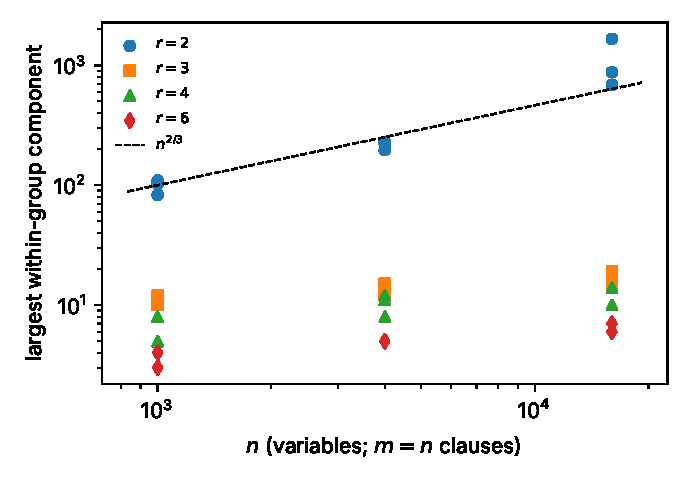
\includegraphics[width=0.55\linewidth]{figures/components.pdf}
\caption{Largest within-group component against $n$ (three seeds per point). At $r = 2$ it is of order $n^{2/3}$; for $r \ge 3$ it grows at most logarithmically.}
\label{fig:components}
\end{figure}

\subsection{What it does and does not imply for the algorithm}

For $r \ge 3$ the group sum $\sum_{u \in X_{t,g}(y_g)} A_{t,g}(u; \vec y)$ factorizes: the measurement $y_g = C_{t,g} u$ is additive across the components of the within-group hypergraph, so the histogram of the group over its measurement box is the convolution of the component histograms, each computable by enumerating a bounded number of assignments. The paper's Step~2, which enumerates all $2^{|S_{t,g}|} \le 2^{2n/r}$ assignments of a group, could be replaced by a convolution whose cost is governed by the number of lanes of the box. Since the paper takes $r \to \infty$, its own regime is deep inside the subcritical range.

This does not improve the theorem. Taking logarithms of the three factors of~(2.11) gives the exponent
\[
n \Bigl[\, \underbrace{\tfrac{R}{Q} \log_2 \tfrac{2Q}{R}}_{T_1\ (\text{Taylor data})} + \underbrace{\tau \log_2(2D+1)}_{T_2\ (\text{measurements})} + \underbrace{\tfrac{1}{r}}_{T_3\ (\text{group})} \Bigr]
\]
up to the paper's constants, and under its parameter choices~(2.19)---$\lambda = \lceil \log_2 n \rceil$, $\nu = \lceil \log_2 \lambda \rceil$, $r = \lfloor \sqrt{\lambda}/\nu^2 \rfloor$, $Q = \lfloor \lambda/(128 \nu) \rfloor$, $R = 4 \lceil \sqrt{\lambda} \rceil$, $\tau = 1/(r\lambda)$, $D = r^{2Q}$---one has, to leading order, $T_1 \approx 256\, \nu^2/\sqrt{\lambda}$, $T_3 \approx \nu^2/\sqrt{\lambda}$ and $T_2 \approx \nu^2/(128 \sqrt{\lambda})$ (Appendix~\ref{app:exponent}). Removing $T_3$ entirely changes the exponent by about one part in $256$ in the limit; at finite $n$ its share is larger (\expShareA\% at $\lambda = 2^{\expFirstPositive}$, the smallest power of two at which every parameter is defined and $T_1 > 0$; \expShareB\% at $2^{32}$; \expShareC\% at $2^{64}$; Appendix~\ref{app:exponent}). The component structure is a fact about the construction, not a route to a faster algorithm; the dominant cost is the Taylor data, $\sum_{j \le q} \binom{n}{j} 2^j$ restricted sums per point, and it is untouched.

\section{Dense versus sparse recombination of group sums}\label{sec:fibre}

The inner sum of~(2.6) for one group and one foreign tuple is a histogram: the weighted number of assignments $u$ of the group at each attained measurement vector $y_g$. If the group splits into components, the histogram is the convolution of the component histograms. Two representations compete. A \emph{sparse dictionary} stores attained vectors only and convolves pairwise. A \emph{dense packed} representation lays the whole measurement box out as lanes of one big integer (Kronecker substitution~\citep{Har09}: lane index $\sum_i (y_i + D_i^-) \prod_{j < i} (2D_j + 1)$, lane width $W$ bits), so that convolving two histograms is one big-integer multiplication and the lanes add exactly as measurements add under concatenation of partial assignments. The packed form is the natural home of the ``additive homomorphism'' in the paper's device; whether it pays is an empirical question about density.

\subsection{Method}

\texttt{fibre\_loop.py} computes the histogram of one group of $k$ variables three ways---\emph{bucket} (enumerate $2^k$ assignments, bucket by $y$), \emph{dict} (components, sparse convolution), \emph{packed} (components, Kronecker lanes, GMP multiplication, lanes reduced modulo $p$ after every product)---on one shared vectorized kernel for enumeration and clause evaluation, so that only the algorithm differs, with all arithmetic exact modulo $p = 2^{31} - 1$ (a production implementation would use several primes and the Chinese remainder theorem; the cost per prime is what is measured). Two instance families are used. The \emph{real design}: the group, forms, shifts and rows of the Section~2.7 construction at $r = 2$, $t = 1$, for a foreign tuple attained by a random assignment. A \emph{synthetic measurement} for $r \ge 3$: the within-group clause structure of a random bounded-occurrence 3-CNF under uniform schedules, with Boolean own inputs, fixed foreign inputs, and $c$ sparse $\pm1$ rows of support three per group. The synthetic family is needed because at these sizes the real construction either couples the group into one component ($r = 2$) or, for $r \ge 3$ at $Q = 2$, produces 9--10 rows per copy and a box larger than $2^k$; the paper's regime of few shared rows exists only at enormous $n$. Every histogram is compared across the three methods; \fibreExactChecks{} of them, with $k \le 12$, are also compared with the exact rational fibre sums of the toy, and every one with $k \le 16$ is recomputed by plain enumeration in the independent check.

\subsection{Results}

\begin{table}[t]
\centering\scriptsize
\caption{The fibre loop three ways (ms). ``comp.'' is the largest component; ``enumerated'' the assignments visited by the component methods against $2^k$; ``attained'' the nonzero lanes of the box (and their fraction of it). Ratios are bucket/packed and dict/packed.}
\label{tab:fibre}
\setlength{\tabcolsep}{4pt}
\begin{tabular}{@{}rrrrrrrrrrr@{}}
\toprule
$k$ & rows & lanes & comp. & enumerated & attained & bucket & dict & packed & b/p & d/p \\
\midrule
\multicolumn{11}{@{}l}{\emph{Real Section 2.7 design, $r = 2$, $t = 1$}}\\
\rows{tables/E3_design.tex}
\midrule
\multicolumn{11}{@{}l}{\emph{Synthetic measurement, $r = 4$, 8 rows}}\\
\rows{tables/E3_synth_r4_rows8.tex}
\midrule
\multicolumn{11}{@{}l}{\emph{Synthetic measurement, $r = 3$, 8 rows}}\\
\rows{tables/E3_synth_r3_rows8.tex}
\midrule
\multicolumn{11}{@{}l}{\emph{Synthetic measurement, $r = 4$, 10 rows}}\\
\rows{tables/E3_synth_r4_rows10.tex}
\bottomrule
\end{tabular}
\end{table}

\begin{figure}[t]
\centering
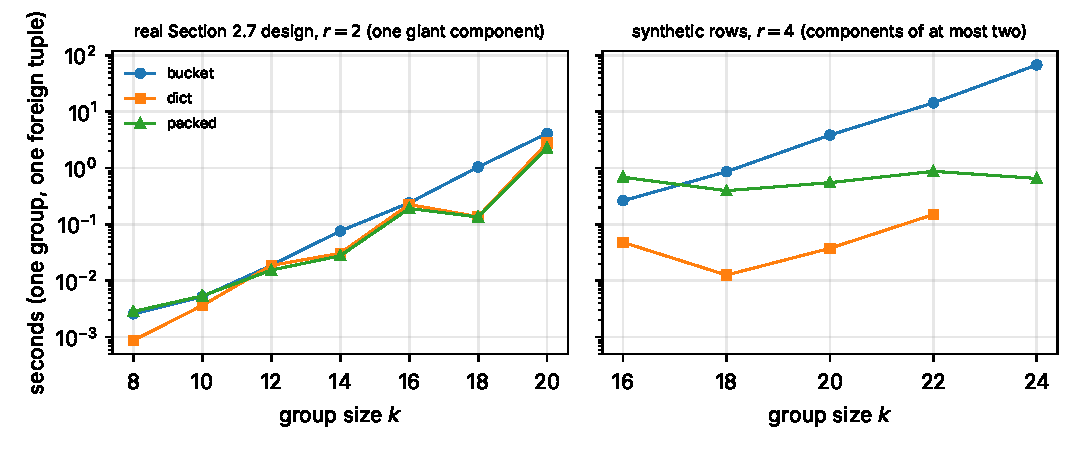
\includegraphics[width=0.95\linewidth]{figures/fibre.pdf}
\caption{Time of the three methods against group size. Left: the real design at $r = 2$, one giant component, where decomposition rarely helps. Right: the synthetic measurement at $r = 4$, components of at most two variables, where enumeration grows as $2^k$ and both component methods stay nearly flat.}
\label{fig:fibre}
\end{figure}

Table~\ref{tab:fibre} and Figure~\ref{fig:fibre} give the numbers. Three readings. First, decomposition is the entire gain: against the $2^k$ enumeration the better of the two component methods wins by \fibreBestSubcritMin--\fibreBestSubcritMax$\times$ for $k \ge 20$ at $r \ge 3$, and by at most \fibreBestRtwoMax$\times$ at $r = 2$, where a win appears only when a small piece splits off the giant component. Second, the packed representation adds nothing over the sparse one: the ratio of dictionary time to packed time is \fibreDictRatioMin--\fibreDictRatioMax{} across the \fibreInstances{} instances, so the packed form is at best \fibreDictRatioMax$\times$ faster (on \fibrePackedFasterCount{} small real-design groups) and at worst \fibrePackedOverDictMax$\times$ slower, because the dense form pays for every lane while only \fibreDensityMin--\fibreDensityMax\% are attained in the synthetic family (Table~\ref{tab:fibre}), and the fraction falls as rows are added, the box being a product of independent ranges in which the attained measurements concentrate near zero. Writing both sides in C would speed them up by similar factors; the ratio is governed by density. Third, the one place a dense form would win is a dense histogram---a single low-range row, such as a cardinality constraint---which is the subject of the next section, and which is served well by the sparse form anyway.

\section{Semiring component caches under side constraints}\label{sec:cache}

\subsection{The engine}

\texttt{constrained\_count.py} is a miniature sharpSAT-style counter (unit propagation; decomposition of the residual formula into connected components; a cache keyed by the canonical residual component; static or dynamic branching) whose cached values are histograms. Given literal weights $w_0[v], w_1[v]$ and $c$ integer rows $a^{(1)}, \dots, a^{(c)}$, it computes
\[
\mathcal H(y) \;=\; \sum_{x \models \F,\ A x = y}\ \prod_{v} w_{x_v}[v] \qquad \text{for every attained } y \in \Zz^c,
\]
by letting a forced literal contribute $w_{x_v}[v]\, z^{x_v a_v}$, a free variable contribute $w_0[v] + w_1[v] z^{a_v}$, and components combine by convolution. With $c = 1$ and $a = (1, \dots, 1)$ this is the weighted count by cardinality; $c = 0$ is plain weighted counting on the same code. By \citet{HD05} the search is a decision-DNNF and by \citet{KVD17} this is its evaluation in the polynomial semiring; nothing in the engine is new, which is the point of the comparison.

The comparison arm is the standard route for an ordinary counter: a functional, counting-preserving sequential-counter encoding of $\sum_v x_v = b$~\citep[after][]{Sin05}, with auxiliaries $s(i,j) \leftrightarrow (\text{at least } j \text{ of } x_1, \dots, x_i)$ for $1 \le j \le \min(i, b+1)$, appended to $\F$ and counted by the same engine with $c = 0$. Propagation, decomposition, cache and branching are shared; only the treatment of the constraint differs.

\subsection{Results}

\begin{table}[t]
\centering\scriptsize
\caption{Independent sets of the $W \times H$ grid by size (static branching order). One histogram run yields every size; each encoding run yields one size $b$. ``comp.'' is the largest component met; the parenthesized ratio is the encoding's time over the whole histogram's.}
\label{tab:grids}
\setlength{\tabcolsep}{3pt}
\begin{tabular}{@{}lrrrrrlp{6.6cm}@{}}
\toprule
grid & $n$ & sizes & ms & nodes & cache/hits & total & encoding, one $b$ \\
\midrule
\rows{tables/E4_grids.tex}
\bottomrule
\end{tabular}
\end{table}

\begin{table}[t]
\centering\scriptsize
\caption{Random 3-CNF (dynamic branching order): the cardinality histogram against the plain weighted count on the same engine, and against the encoding of one $b$.}
\label{tab:random}
\setlength{\tabcolsep}{3pt}
\begin{tabular}{@{}rrlrrrrrp{5.4cm}@{}}
\toprule
$n$ & $m$ & weights & entries & hist.\ ms & nodes & plain ms & hist/plain & encoding, one $b$ \\
\midrule
\rows{tables/E4_random.tex}
\bottomrule
\end{tabular}
\end{table}

\begin{figure}[t]
\centering
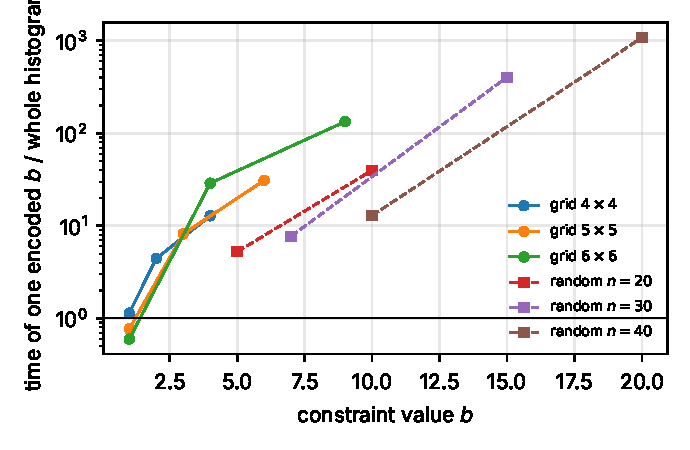
\includegraphics[width=0.55\linewidth]{figures/encoding.pdf}
\caption{Cost of one CNF-encoded cardinality value $b$ relative to the whole histogram computed by the semiring cache, on the same engine.}
\label{fig:encoding}
\end{figure}

Tables~\ref{tab:grids} and~\ref{tab:random} and Figure~\ref{fig:encoding} give the numbers; every grid total equals OEIS~A006506~\citep{OEIS,CW98}, every histogram with $n \le 20$ equals brute force, and every encoded count equals its histogram entry. Three readings. The histogram-valued cache computes the entire histogram at \histOverPlainMin--\histOverPlainMax$\times$ the cost of one plain count: the search and the cache are identical and only the stored values change; on the $6 \times 6$ grid a pseudo-Boolean row with $a_v \in \{1,2,3\}$ (\multirowPBentries{} values) costs \multirowPB{} ms and two rows (left-half and right-half counts, \multirowTwoEntries{} pairs) \multirowTwo{} ms against \gridSixSixMs{} ms for the cardinality row. The encoding route multiplies the cost of a single $b$ by up to \encRatioGridMax$\times$ on grids and \encRatioRandomMax$\times$ on random 3-CNF, growing with $b$ and $n$, because the counter chain couples every variable: the largest component grows from $n$ to $n$ plus the auxiliaries (36 to \gridSixEncComp{} on the $6 \times 6$ grid at the mode, where the ratio is \gridSixEncRatio$\times$; 40 to \encFortyTwentyComp{} at $n = 40$, $b = 20$, where one encoded value takes \encFortyTwentySeconds{} s and \encFortyTwentyNodes{} nodes against \histFortyMs{} ms for all \histFortyEntries{} values, a ratio of \encFortyTwentyRatio$\times$), decomposition disappears, and the cache fills with states that differ only in their prefix count. This is the known weakness of CNF-encoded cardinality constraints for counters and the known remedy; for grid independent sets the remedy reduces to the transfer-matrix method of \citet{CW98}, which is also what our independent check uses. The production compilers~\citep{LM17} produce d-DNNF on which the same semiring evaluation is a post-processing step; what we have not measured, for want of those tools in our environment, is the constant-factor comparison between a top-down histogram cache and compilation followed by evaluation.

\section{Discussion}\label{sec:discussion}

\paragraph{What an additive measurement buys.} The three regimes line up on one axis. With no measurement, the oblivious sampler of Section~\ref{sec:oblivious} cannot see the formula and fails on a forced assignment. With lossy, bounded, algebraically deformed measurements, the algorithm of \citet{OpenAI26} separates groups at the cost of an interpolation whose Taylor-data term dominates its exponent; its construction has more structure than its analysis uses (Section~\ref{sec:components}), and the natural dense representation of its group sums buys nothing at reachable densities (Section~\ref{sec:fibre}). With an exact additive side measurement carried through a component cache, practical constrained counting gets its histogram nearly for free (Section~\ref{sec:cache}); that is the generating-function structure of algebraic model counting, and it was known. The homomorphism that pays, in the end, is the additivity of the side constraint across disjoint components, in sparse form.

\paragraph{Verification and comprehension of AI-generated proofs.} The Lean development accompanying \citet{OpenAI26} certifies the top-line statement with far more authority than any computation at $n \le 14$. What the executable model adds is of a different kind: a reader can print the design at $t = 1$ and $t = 2$ (Section~\ref{sec:auxexample}), see that a measurement is $x_3 - x_{12}$, see an input become $-\tfrac12 T x_3$, and see $H(1) = \auxTwelveHone$ agree with a brute-force sum. We suggest that releases of machine-generated mathematics would benefit from such models alongside their formalizations, and we release ours as a contribution to the community revision of this manuscript~\citep{OAIrepo}.

\paragraph{Limitations.} The toy certifies identities and constructions at sizes where every quantity is enumerable; it says nothing about asymptotics. The greedy schedules of the aux design replace the paper's derandomized balancing, whose hypothesis fails at toy sizes. The synthetic measurement of Section~\ref{sec:fibre} is a stand-in for a regime the real construction reaches only at astronomical $n$. The counter of Section~\ref{sec:cache} is a miniature in Python; its absolute times are not those of a production tool, and the ratios it measures are between two arms of the same engine. All wall-clock times are single runs on shared virtual hardware; the deterministic counts beside them (nodes, assignments, lanes, cache entries) carry the argument.

\paragraph{Future work (speculative, not a result).} The author's prior work on computing on compressed data suggests asking whether a component cache can hold its histograms in a compressed representation that still admits convolution without decompression. Section~\ref{sec:fibre} shows that dense lane packing is not that representation at the densities seen here; a sparse, additively homomorphic encoding of attained measurement vectors would have to beat a hash map on both time and memory to matter, and we know of no evidence that it does. We record the question and no claim.

\section{Reproducibility}\label{sec:repro}

\paragraph{Code and dataset.} The repository, \url{https://github.com/chelsinchaos/measurement-indexed-counting}, contains \texttt{measurement\_toy.py} (the executable model; standard library only), \texttt{fibre\_loop.py} (Section~\ref{sec:fibre}; NumPy and gmpy2), \texttt{constrained\_count.py} (Section~\ref{sec:cache}; standard library only), \texttt{run\_all.py} (regenerates the dataset), \texttt{independent\_check.py} (verification run~2), and \texttt{make\_tables.py} (produces every table, figure and number in this paper from the dataset). The dataset holds every formula in DIMACS with its generator and seed, every design of the toy as JSON, the results of the four experiments as JSON with environment metadata, the logs, and a manifest with the SHA-256 of each of its \datasetFiles{} files. Environment: Python \envPython, NumPy \envNumpy, gmpy2 \envGmpy, \envCpus{} virtual CPUs, \envPlatform.

\paragraph{Three verification runs.} \emph{Run 1} is the generation itself, which aborts on any failed internal check: the measurement algorithm against brute force at every design point, $H(0)$ against the solution counter, the three fibre-loop methods against each other and against exact rational fibre sums, grid totals against OEIS~A006506, histograms against brute force at $n \le 20$, and every encoded count against its histogram entry. \emph{Run 2} (\texttt{independent\_check.py}) recomputes the results by different algorithms written separately from the generating code: the deformed count $H(T)$ as an explicit polynomial by symbolic brute force over all assignments (which also confirms every recorded Taylor coefficient and re-tests the design conditions with a fresh rank routine); component sizes by breadth-first search instead of union-find; fibre histograms with $k \le 16$ by plain enumeration from the stored clauses, forms, shifts and rows; grid histograms by a transfer-matrix dynamic programme that never decomposes or caches; and random-3-CNF histograms by exhaustive DPLL enumeration that visits every model. It passed \indepPassed{} of \indepChecks{} checks. \emph{Run 3} is an audit by an agent with no access to the development history. It re-executed the generation in quick mode in a clean directory (quick mode skips the four longest runs: the toy at $n = 14$ with $q = 1$, the component statistics at $n = 16{,}000$, the two $k = 24$ fibre instances and the encoding at $n = 40$, $b = 20$; the first and last of these are covered by Run~2's symbolic expansion and exhaustive enumeration, while the $n = 16{,}000$ statistics and the $k = 24$ timings rest on the single generation run), found zero differences in deterministic quantities, re-ran the independent check (74 of 74), recomputed 45 of this paper's generated numbers from the raw JSON with its own code, and found six defects in the prose of the first draft, all corrected in this version. Its report is \texttt{VERIFICATION.md} in the repository.

\section*{Acknowledgements}
The implementation, experiments and drafting were carried out with Claude (Anthropic) as an AI research assistant under the author's direction; the author is responsible for all content and for any errors. The manuscript studied here was made available by OpenAI under the Apache-2.0 licence of its repository.

\bibliographystyle{plainnat}
\bibliography{refs}

\appendix

\section{The Section 2.7 construction, step by step at $r = 2$, $Q = 2$, $R = 2$}\label{app:aux}

We record the construction as implemented, with the quantities that the reader can recompute by hand. Groups are $\{1, 2\}$ and points are $t \in \{1, 2\}$.

\emph{Step 1 (coordinates).} $B = (\{1,2\} \times \{1,2\})^2$, $D = 16$. An index $u = ((a_u(1), d_u(1)), (a_u(2), d_u(2)))$ records, at each point, the group $a_u(t)$ of the coordinate and the group $d_u(t)$ of the clause that will read it. The swap $\Pi_s$ exchanges the two entries of pair $s$.

\emph{Step 2 (the constant matrix).} $p = (r-1)/(2r) = 1/4$, $Qp = 1/2$, $A_0 = \lfloor Qp - (R-1)/2 \rfloor = 0$, $I = \{0, 1\}$, and $f$ is the line through $(0, 1)$ and $(1, -1)$: $f(j) = 1 - 2j$. With $W_0 = \tfrac12\sum_s (I - \Pi_s)$ and $V_0 = \Pi_1 \Pi_2$,
\[
M_0 \;=\; V_0 f(W_0) \;=\; \Pi_1\Pi_2\bigl(-I + \Pi_1 + \Pi_2\bigr) \;=\; \Pi_1 + \Pi_2 - \Pi_1\Pi_2 .
\]
Per position the swap has eigenvectors $e_{11}, e_{22}, e_{12} + e_{21}$ (eigenvalue $+1$) and $e_{12} - e_{21}$ (eigenvalue $-1$); the product basis of $B$ has $j \in \{0, 1, 2\}$ positions with eigenvalue $-1$, and $M_0 \psi = (-1)^j f(j) \psi$, which equals $\psi$ for $j \in I$ and $-3\psi$ for $j = 2$. Fifteen of the sixteen basis vectors are fixed; the remaining one, $(e_{12} - e_{21}) \otimes (e_{12} - e_{21})$, is the single row of $C$, supported on the four coordinates with both pairs in $\{(1,2), (2,1)\}$.

\emph{Step 3 (the rows).} For $u$ and a nonzero $M_0[u, w]$, $E_{u,w} = \{t : a_w(t) \ne d_u(t)\}$; for $w = \Pi_1 u$ this is empty at $t = 1$ and contains $t = 2$ exactly when $a_u(2) \ne d_u(2)$, so $|E_{u,w}| \le 1 = R - 1$. Then
\[
\angles{\vec P_u(T), \zeta} \;=\; \bigl((I - M_0)\zeta\bigr)_u + \sum_{w} M_0[u,w]\, \prod_{s \in E_{u,w}} \Bigl(1 - \frac{T}{s}\Bigr)\, \zeta_w ,
\]
which equals $\zeta_u$ at $T = 0$; at $t = 1$ the surviving $\zeta_w$ have $a_w(1) = d_u(1)$, i.e.\ lie in the assigned group, and the first term is a multiple of the measurement $C\zeta$. For $u = ((1,2),(1,2))$ one obtains $\angles{\vec P_u(T), \zeta} = [\zeta_u - \zeta_{\Pi_1 u} - \zeta_{\Pi_2 u} + \zeta_{\Pi_1\Pi_2 u}] + (1 - T/2)\zeta_{\Pi_1 u} + (1 - T)\zeta_{\Pi_2 u} - \zeta_{\Pi_1 \Pi_2 u}$: collecting coefficients, the row is $\zeta_u - \tfrac{T}{2}\zeta_{\Pi_1 u} - T\zeta_{\Pi_2 u}$, which after the substitution of Step~4 is exactly the example form $\auxTwelveExampleForm$ of Section~\ref{sec:auxexample}; at $t = 1$ the bracket is the shared measurement and the rest reads $\tfrac12 \zeta_{\Pi_1 u} - \zeta_{\Pi_1\Pi_2 u}$ from group~2.

\emph{Step 4 (substitution).} Variables receive schedules $a_v \in [2]^2$ in a balanced round robin; clauses receive $d_e \in [2]^2$ by a greedy choice that minimizes the maximum label multiplicity $h$; occurrence $(e, v)$ gets label $u(e,v) = ((a_v(1), d_e(1)), (a_v(2), d_e(2)))$ and a copy $j(e,v) \in [h]$; copy $j$ holds $X_v$ at coordinate $u(e,v)$ and zero elsewhere; and $\vec P_{e,v}(T)$ is $\vec P_{u(e,v)}(T)$ applied to copy $j(e,v)$. The measurements are $C$ applied to each copy, split by group into the rows of $C_{t,g}$ shown in Section~\ref{sec:auxexample}. Every property is checked numerically as the objects are built, and condition~(2.5) is verified at every point by solving for $\vec\lambda_{e,v,h}$.

\section{The exponent under the paper's parameters}\label{app:exponent}

With $\lambda = \lceil \log_2 n \rceil$ and $\nu = \lceil \log_2 \lambda \rceil$, the choices~(2.19) give $R/Q \approx 4\sqrt{\lambda} \cdot 128\nu/\lambda = 512\nu/\sqrt{\lambda}$ and $\log_2(2Q/R) \approx \log_2\bigl(\sqrt{\lambda}/(256\nu)\bigr) = \tfrac12 \log_2 \lambda - \log_2 \nu - 8$, whose leading term is $\nu/2$; hence $T_1 = (R/Q)\log_2(2Q/R) \approx 256\,\nu^2/\sqrt{\lambda}$. Next $T_3 = 1/r \approx \nu^2/\sqrt{\lambda}$. Finally $T_2 = \tau \log_2(2D + 1) \approx (1/(r\lambda)) \cdot 2Q \log_2 r \approx (\nu^2/\lambda^{3/2}) \cdot (\lambda/(64\nu)) \cdot \log_2 r$ with $\log_2 r \approx \tfrac12 \log_2 \lambda - 2\log_2 \nu$, leading term $\nu/2$, so $T_2 \approx \nu^2/(128\sqrt{\lambda})$. Thus $T_1 : T_3 : T_2 \approx 256 : 1 : 1/128$ to leading order, and deleting $T_3$ changes $T_1 + T_2 + T_3$ by a factor $1 - 1/257 + O(1/\nu)$. The lower-order terms we dropped ($-\log_2\nu - 8$ against $\nu/2$) are not small at any $n$ one would write down, which is one more way of saying that the regime is asymptotic. With the integer choices of~(2.19) the parameters are not even all defined for small $\lambda$: $r = \lfloor \sqrt{\lambda}/\nu^2 \rfloor$ is $0$ at $n = 10^{100}$ and at $n = 10^{1000}$, and $T_1$ first becomes positive at $\lambda = \expThresholdLambda \approx 2^{\expThresholdLog}$, so $\lambda = 2^{\expFirstPositive}$ (that is, $n = 2^{2^{\expFirstPositive}}$) is the smallest power of two with $T_1 > 0$. Evaluating the three terms exactly at $\lambda = 2^k$: $T_1/T_3 = \expRatioA, \expRatioB, \expRatioC, \expRatioD, \expRatioE$ and the share $T_3/(T_1 + T_2 + T_3)$ is $\expShareA\%, \expShareB\%, \expShareC\%, \expShareD\%, \expShareE\%$ for $k = 26, 32, 64, 128, 512$, against the limit \expShareLimit\%. The conclusion that $T_1$ dominates survives at every $\lambda$ for which the terms are defined and positive; the figure ``one part in $256$'' is the limit.

\end{document}
